\documentclass{beamer}

% This file is a solution template for:

% - Giving a talk on some subject.
% - The talk is between 15min and 45min long.
% - Style is ornate.



% Copyright 2004 by Till Tantau <tantau@users.sourceforge.net>.
%
% In principle, this file can be redistributed and/or modified under
% the terms of the GNU Public License, version 2.
%
% However, this file is supposed to be a template to be modified
% for your own needs. For this reason, if you use this file as a
% template and not specifically distribute it as part of a another
% package/program, I grant the extra permission to freely copy and
% modify this file as you see fit and even to delete this copyright
% notice. 


\mode<presentation>
{
  \usetheme[height=12mm]{Rochester}
  % or ...%

  \setbeamercovered{transparent}
%  % or whatever (possibly just delete it)
}


\usepackage[brazil]{babel}
% or whatever

% or whatever
%\usepackage{graphics}
\usepackage{times}
\usepackage[utf8]{inputenc}
\usepackage{url}
\usepackage{amsmath}
\usepackage{cancel}


\newcommand{\nektar}{\ensuremath{\mathcal{N}\varepsilon \kappa \tau \alpha r}}
\newcommand{\ordem}[1]{ \ensuremath{\mathcal{O}[#1]}}
\newcommand{\pr}[1]{\ensuremath{ \mathbf{#1}}}    % \pr vem de preto
\newcommand{\etal}{\emph{et al.}}
\newcommand{\jac}[4]{ \ensuremath{ P_{#2}^{#3,#4}(#1) }}
\newcommand{\der}[2]{\ensuremath{ \frac{\partial #1}{\partial #2}}}
\newcommand{\convect}[2]{\ensuremath{ #1 \cdot \nabla #2}}
\newcommand{\R}{\ensuremath{ Re }}
\newcommand{\St}{\ensuremath{ St }}
\newcommand{\cpb}{\ensuremath{ C_{pb}}}
\newcommand{\transf}[3]{\ensuremath{ \int_{-\infty}^\infty #3\: e^{i #2 #1}\: d #2}}
\newcommand\clrms{\ensuremath{\sqrt{\overline{C_L^2}}}}
\newcommand{\epseudo}{\ensuremath{ \epsilon-\text{pseudospectro}}}
\newcommand{\lra}{\ensuremath{\longrightarrow}}

\newcommand{\wt}[1]{\ensuremath{\widetilde{#1}}}
\newcommand{\mcal}[1]{\ensuremath{\mathcal{#1}}}

\newcommand{\ol}[1]{\ensuremath{\overline{#1}}}
\newcommand{\us}{\ensuremath{u_*}}

\newcommand{\p}[1]{\ensuremath{ \mathbf{#1}}}    % \pr vem de preto
\newcommand{\qrq}{\ensuremath{\quad\lra\quad}}
\newcommand{\qqrq}{\ensuremath{\qquad\lra\qquad}}
\newcommand{\pd}{\ensuremath{\partial}}
\newcommand{\bigO}[1]{\ensuremath{\mathcal{O}\left(#1\right)}}


\title{Camada limite}


\author{Paulo Jabardo}

\titlegraphic{
\includegraphics[width=4cm]{figuras/logo-ipt.png}}%}
%   \includegraphics[width=2cm]{fig
%}
\date{24-11-2023}





\begin{document}
\maketitle

\begin{frame}{Navier-Stokes}
\[
\frac{\pd\p{u}_*}{\pd t_*} + \p{u}_*\cdot\nabla_*\p{u_*} = -\frac{P_0}{\rho U_0^2}\nabla_* p_* + \frac{1}{Re}\nabla_*^2\p{u}_* \qquad \nabla_*\cdot\p{u}_* = 0
\]
\[
\nabla \cdot \p{u}_* = 0
\]

Primeira tentação: $Re\to\infty$ - \emph{desprezar o termo difusivo}

\end{frame}

\begin{frame}{Camada Limite}
  \centering
  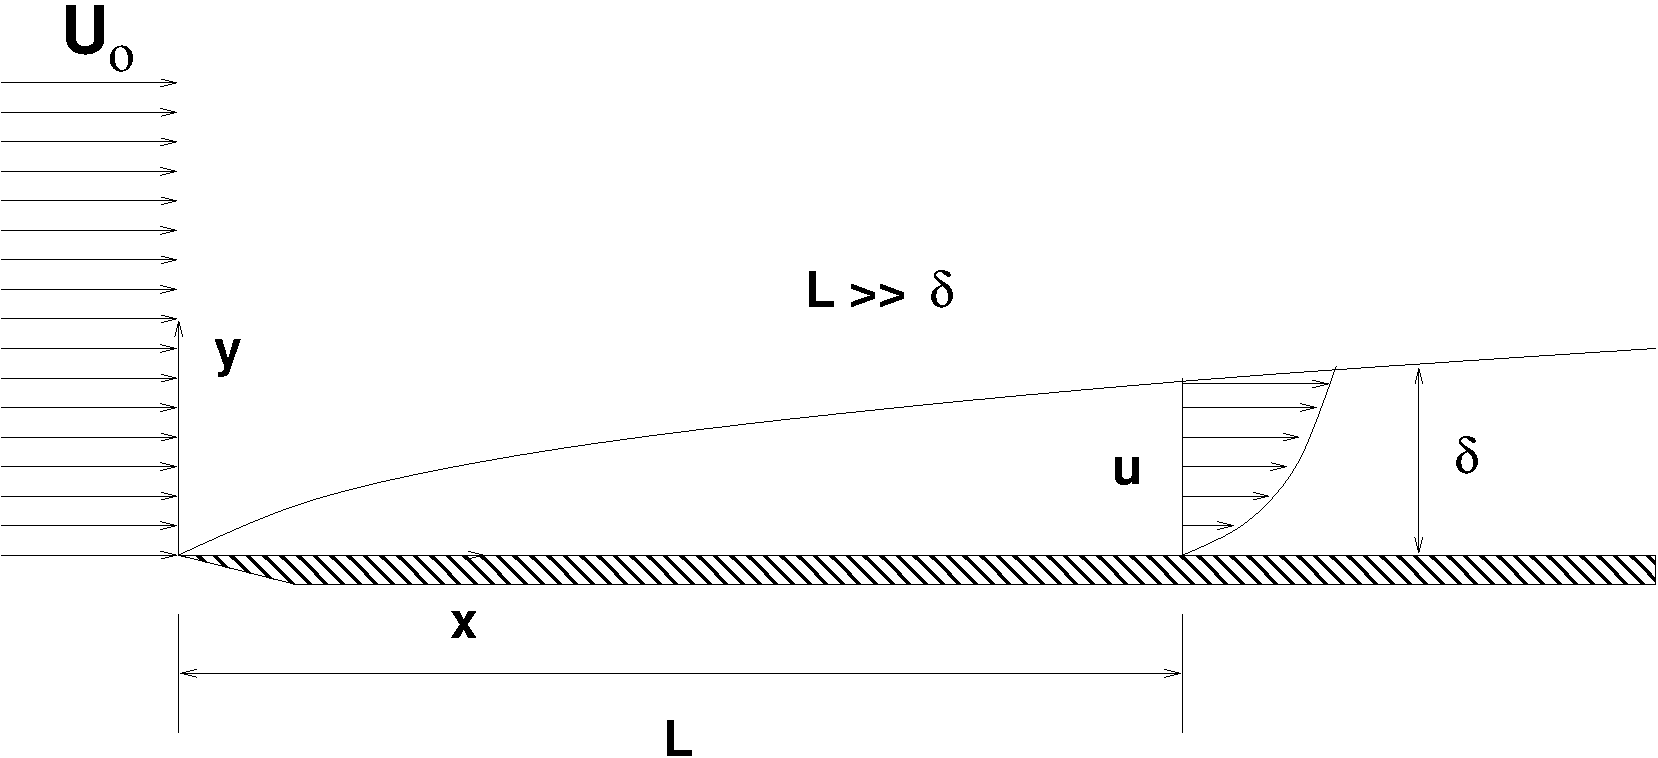
\includegraphics[width=0.85\textwidth]{./figuras/camada-limite.pdf}
\end{frame}

\begin{frame}{Navier-Stokes}
  \[
\begin{matrix}
\frac{\pd\p{u}}{\pd t}& +& \p{u}\cdot\nabla\p{u}& = &-\frac{1}{\rho}\nabla p& +& \nu\nabla^2\p{u}\\
\bigO{\frac{U_0^2}{L}}& & \bigO{\frac{U_0^2}{L}} &  & \bigO{\frac{U_0^2}{L}}&  & \xcancel{\bigO{\nu\frac{U_0}{L^2}}} \\
 & & & & & & \bigO{\nu\frac{U_0}{\delta^2}}\\
\end{matrix}
  \]

  Aí temos a estimativa

  \[
  \frac{U_0^2}{L} \sim \nu\frac{U_0}{\delta^2} \qrq \frac{\delta}{L} \sim \sqrt{\frac{1}{Re}}
  \]

\end{frame}

\begin{frame}{Navier-Stokes 2D, regime permanente}
  \begin{align*}
    u_*\frac{\partial u_*}{\partial x_*} + v_*\frac{\partial u_*}{\partial y_*} &= 
    -\frac{\partial p_*}{\partial x_*} + \frac{1}{Re} \left( \frac{\partial^2 u_*}{\partial x_*^2} + \frac{\partial^2 u_*}{\partial y_*^2}\right) \\
    u_*\frac{\partial v_*}{\partial x_*} + v_*\frac{\partial v_*}{\partial y_*} &= 
    -\frac{\partial p_*}{\partial y_*} + \frac{1}{Re} \left( \frac{\partial^2 v_*}{\partial x_*^2} + \frac{\partial^2 v_*}{\partial y_*^2}\right) \\
    \frac{\partial u_*}{\partial x_*} &+ \frac{\partial v_*}{\partial y_*} = 0\\
  \end{align*}

\end{frame}


\begin{frame}{Escalas do problema}
  Hipóteses: 2D, regime permanente
  \begin{itemize}
  \item $x \sim L$
  \item $y \sim \delta$
  \item $u \sim U_0$
  \item $v \sim ???$
  \item $p \sim ???$
  \end{itemize}

  \[
  \delta_* = \frac{\delta}{L}
  \]
  
\end{frame}

\begin{frame}{Escalas do problema}
  Equação da continuidade:
  \[
  \frac{\partial u}{\partial x} + \frac{\partial v}{\partial y} = 0 \qrq \frac{U_0}{L} + \frac{V_0}{\delta} \sim 0 \qrq V_0 \sim \frac{\delta}{L} \times U_0
  \]

\[
\begin{matrix}
 u_*&\frac{\partial u_*}{\partial x_*} + &v_*&\frac{\partial u_*}{\partial y_*} =& 
-\frac{\partial p_*}{\partial x_*} + &\frac{1}{Re} &\left( \frac{\partial^2 u_*}{\partial x_*^2}\right. +& \left.\frac{\partial^2 u_*}{\partial y_*^2}\right) \\
1 & \frac{1}{1} & \delta^* & \frac{1}{\delta^*} & ? & \ll 1 & 1 & \frac{1}{\delta_*^2} \\
\end{matrix}
\]

\[
\frac{1}{Re} \left( \frac{\partial^2 u_*}{\partial x_*^2}\right. + \left.\frac{\partial^2 u_*}{\partial y_*^2}\right)\sim 1\qrq Re \sim \frac{1}{\delta_*^2}
\]

\end{frame}

\begin{frame}{E na direção y?}
\[
\begin{matrix}
u_*&\frac{\partial v_*}{\partial x_*} + &v_*&\frac{\partial v_*}{\partial y_*} =& 
-\frac{\partial p_*}{\partial y_*} + &\frac{1}{Re} &\left( \frac{\partial^2 v_*}{\partial x_*^2}\right. +& \left.\frac{\partial^2 v_*}{\partial y_*^2}\right) \\
 1 & \delta_* & \delta_* & 1 & ? & \delta_*^2 & \delta_* & \frac{1}{\delta_*} \\
\end{matrix}
\]
de modo que 
\[
\frac{\partial p_*}{\partial y_*} = \bigO{\delta_*} \approx 0
\]
Ou seja:
\[
p_* = p_*(x)
\]

\vspace{1cm}
A pressão é imposta de fora na camada limite!!!
\end{frame}

\begin{frame}{O que conseguimos?}
    \begin{align*}
    u_*\frac{\partial u_*}{\partial x_*} + v_*\frac{\partial u_*}{\partial y_*} &= 
    -\left[\frac{dp_*}{dx_*}\right] + \frac{1}{Re} \frac{\partial^2 u_*}{\partial y_*^2} \\
    p_* &= p_*(x_*)\\
    \frac{\partial u_*}{\partial x_*} + \frac{\partial v_*}{\partial y_*} &= 0\\
  \end{align*}

    Equação elíptica $\lra$ equação parabólica.
\end{frame}
\begin{frame}{Solução de Blasius}
  Será que $\delta$ é sufuciente? Para $L$ sim mas e para $x < L$? O certo:
  \[
  \delta = \delta(x)
  \]

  Então temos uma escala que muda com $x$:
\[
y_* = \frac{y}{\delta} = \frac{y}{\delta(x)} = \eta
\]
O campo de velocidade é dados por:
\[
\frac{u}{U_0} = g\left[\frac{y}{\delta(x)}\right] = g(\eta)
\]
 
\end{frame}

\begin{frame}{Função corrente $\psi$}
  \begin{multline*}
    \psi = U_0 \delta(x) f(\eta) \qquad \frac{u}{U_0} = \frac{\partial\psi}{\partial y}=f'(\eta)=g(\eta) \\
    \frac{v}{U_0} =-\frac{\partial\psi}{\partial x} = \frac{d\delta}{dx}\left(\eta f' - f\right)\\
\end{multline*}
Mas quanto vale $\delta(x)$? Já calculamos uma estimativa antes!
\[
  \frac{\delta(x)}{x} = \sqrt{\frac{2}{Re_x}} \qrq \delta(x) = \sqrt{\frac{\nu x}{U_0}}
  \]

\end{frame}

\begin{frame}{Equações da Camada Limite}
  \[
\frac{\partial u}{\partial x} = -U_0\eta f'' \frac{d\delta}{dx}, 
\quad \frac{\partial u}{\partial y} = \frac{U_0 \cdot f''}{\delta}, \quad \frac{U_0 \cdot f'''}{\delta^2}
\]
chega-se à seguinte equação:
\[
\frac{U_0^2}{\delta}\frac{d\delta}{dx} ff'' + \frac{\nu U_0}{\delta^2}f''' = 0
\]
\end{frame}

\begin{frame}{Auto-semelhança}
Se esta equação não depende de $x$ temos auto-semelhança!
  \[
\frac{U_0^2}{\delta}\frac{d\delta}{dx} ff'' + \frac{\nu U_0}{\delta^2}f''' = 0
\]

Para isso
  \[
\frac{U_0^2}{\delta}\frac{d\delta}{dx} \propto \frac{\nu U_0}{\delta^2} \qrq \delta^2 \propto \frac{\nu x}{U_0} + const \qrq \delta = \sqrt{\frac{2 \nu x}{U_0}}
\]

\end{frame}

\begin{frame}{Solução de Blasius}
  \[
ff'' + f''' = 0
\]
com as seguintes condições de contorno:
\[
f = f' = 0 \quad\text{em}\quad \eta = 0
\]
\[
f' \lra 1 \quad\text{quando}\quad \eta\lra\infty
\]

\end{frame}

\begin{frame}{Limitações}
  \[
\frac{\delta}{x} = \frac{1}{x}\cdot \sqrt{\frac{2 \nu x}{U_0}} = \sqrt{\frac{2}{Re_x}}
\]

O que acontece quando $Re_x\to 0$? Singular

Camada limite:
\begin{itemize}
\item Duas escalas bem distintas $\delta$, $L$
\item Quando $Re_x$ é pequeno, $\delta \sim x$
\end{itemize}

\end{frame}

\begin{frame}{Exercícios}
  \begin{itemize}
  \item Como resolver a solução de Blasius em um CFD tradicional? Qual a malha e as condições de contorno
  \item Tutorial do programa SU2 \url{https://su2code.github.io/}
  \item Programa para solução de camada limite TEXSTAN \url{http://texstan.com/}
    \begin{itemize}
    \item ``Convective Heat and Mass Transfer'' de Kays e Crawford
    \item Longa história
    \item Muito rápido
    \item Bom lugar para testar modelos de turbulência
    \item Alguém quer ajudar a desenvolver uma alternativa livre?
    \end{itemize}
  \end{itemize}
  
\end{frame}

\end{document}


\begin{frame}{}
\end{frame}

\begin{itemize}
\end{itemize}
